\documentclass[../Main.tex]{subfiles}
\begin{document}

\section{Marco teórico}
\subsection{Natural language processing (NLP)}
\begin{justify}
El procesamiento del lenguaje natural es un área integral de la informática en la que se utilizan ampliamente el aprendizaje automático y la lingüística computacional. Este campo se ocupa principalmente de hacer que la interacción humana y la computadora sea fácil pero eficiente. La máquina aprende la sintaxis y el significado del lenguaje humano, lo procesa y le da la salida al usuario. El área de PLN implica la creación de sistemas informáticos para realizar tareas significativas con el lenguaje natural y comprensible para los humanos \cite{15}. 
\end{justify}\par
\begin{justify}
La razón por la que el procesamiento del lenguaje natural es tan importante en el futuro es que ayuda a construir modelos y procesos que toman trozos de información como entrada y en forma de voz o texto o ambos y los manipulan según el algoritmo dentro de la computadora. Por lo tanto, la entrada puede ser voz, texto o imagen, donde la salida de un sistema de PLN puede procesarse tanto en voz como en texto escrito \cite{15} .
\end{justify}\par
\begin{justify}
Algunos de los diferentes algoritmos desarrollados para aumentar la eficiencia del procesamiento del lenguaje en forma de texto son:
\end{justify}\par
\begin{itemize}
	\item Memoria a largo plazo a corto plazo:\par
    LSTM significa memoria a corto plazo \cite{16}. La red neuronal recurrente es el elemento principal del modelo LSTM. La red neuronal recurrente es un fragmento de red neuronal que puede recordar valores. LSTM es un tipo especial de red neuronal recurrente que puede recordar la entrada anterior en un intervalo de tiempo arbitrario y predecir la salida. Se utiliza para entrenar la máquina mediante conjuntos de entrada. Es uno de los modelos de aprendizaje en aprendizaje automático que se utiliza ampliamente en el procesamiento del lenguaje natural.
    
	\item Secuencia 2 Modelo de secuencia (Seq2Seq): \par
    El modelo tradicional seq2seq contiene dos redes neuronales recurrentes, es decir, una red codificadora y una red decodificadora \cite{17}.
    \par
    \begin{figure}[H]
	\begin{Center}
		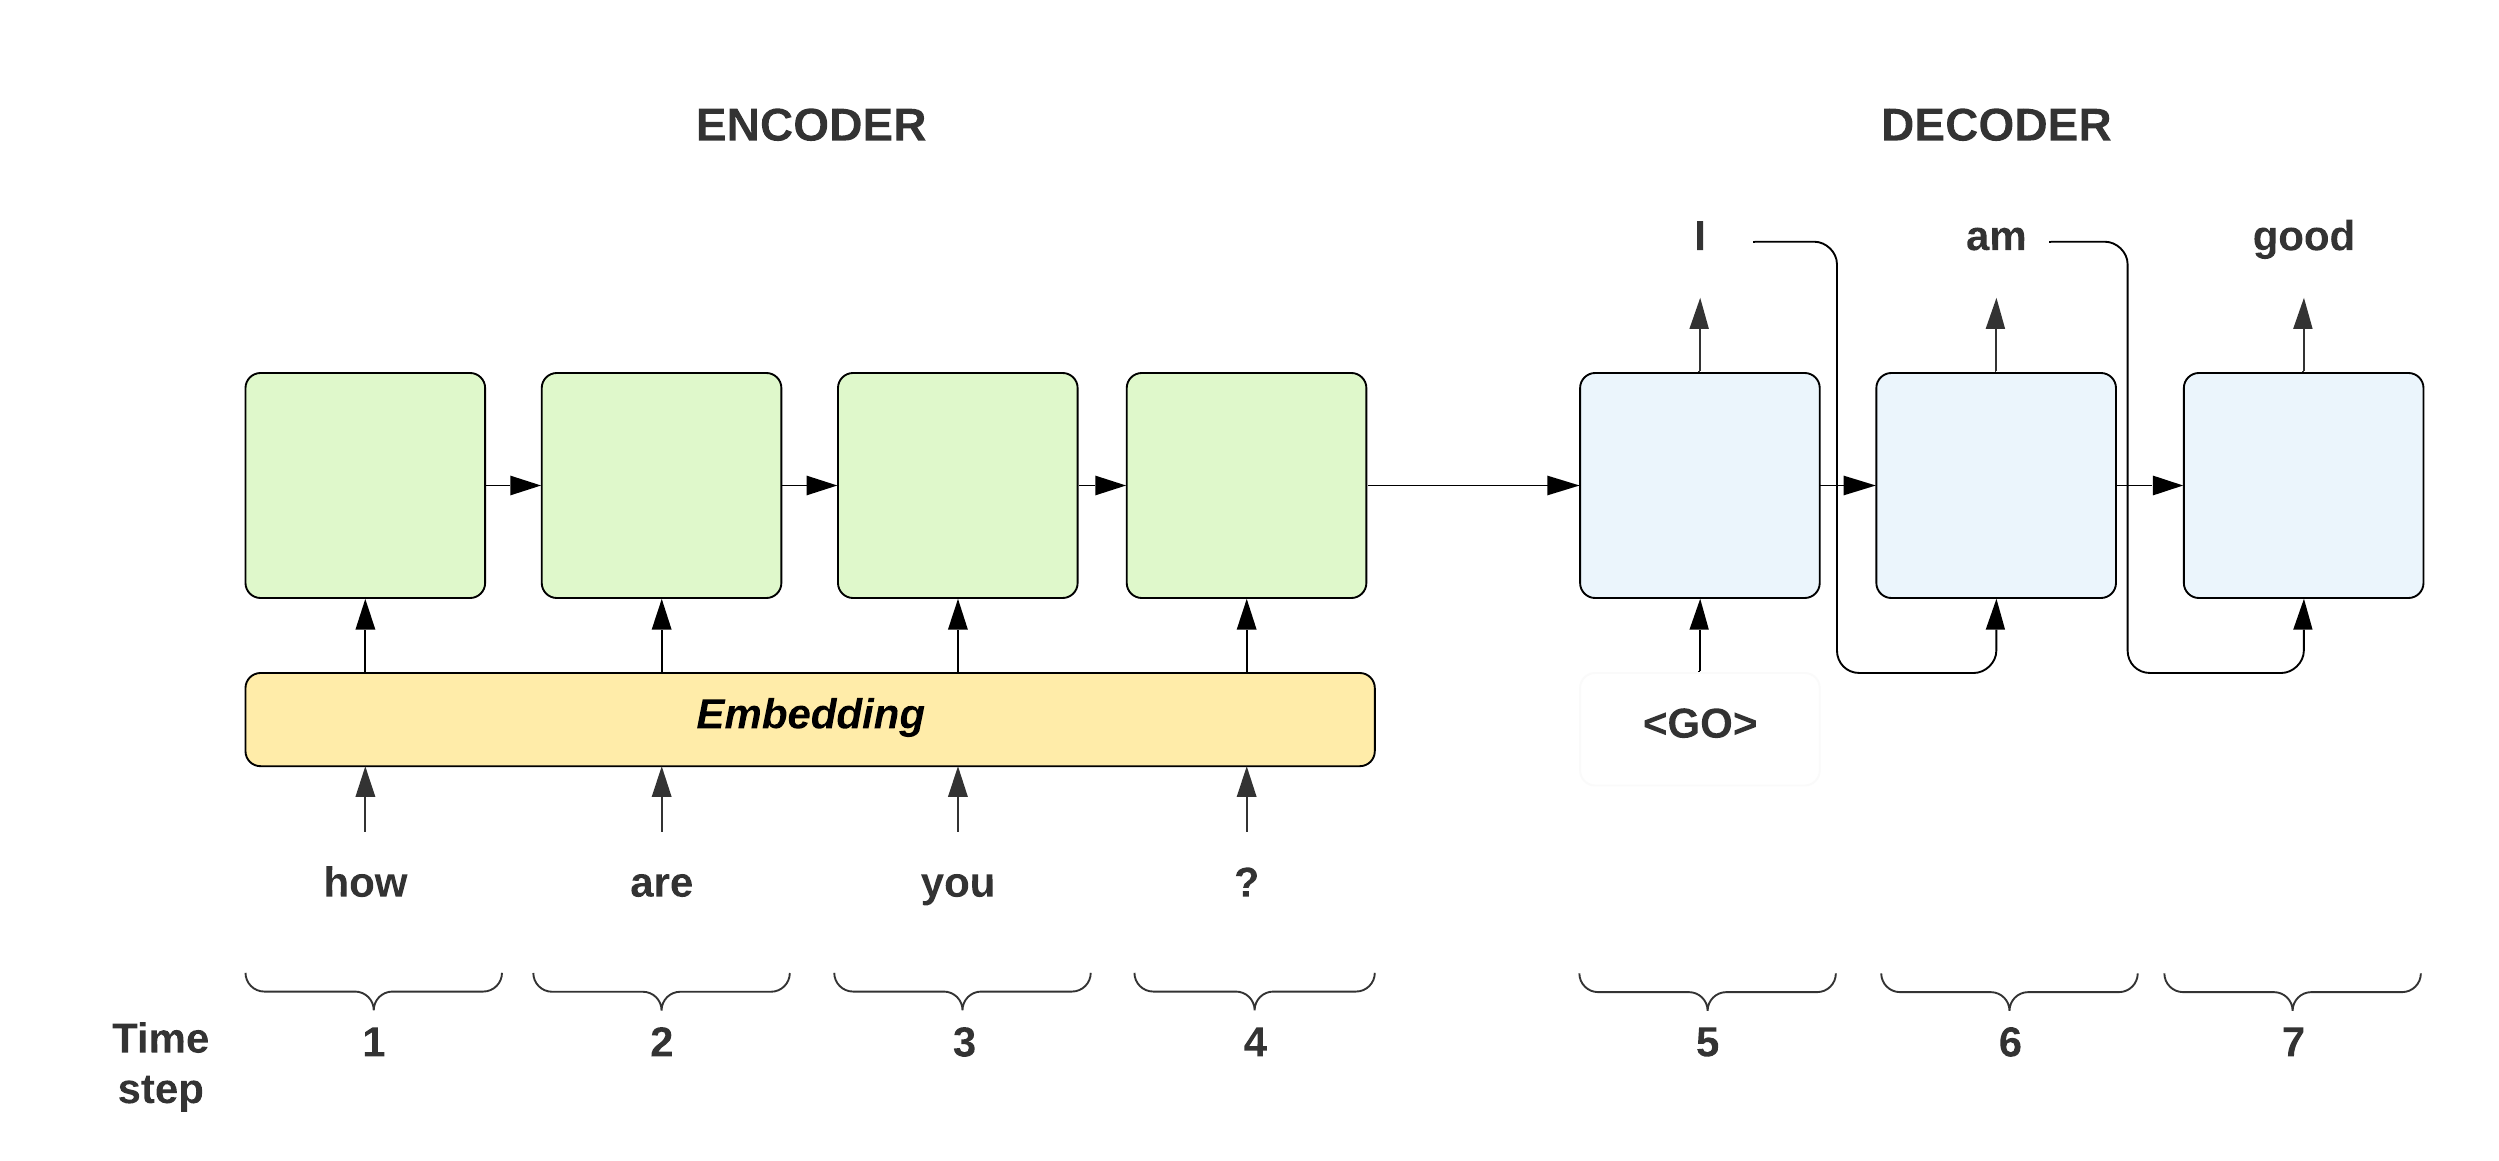
\includegraphics[width=6.4in,height=3in]{Images/encoder_decoder.png}
	    \caption{Encoder Decoder structure}
	    Fuente: Elaboración propia
        \label{fig:section}
	\end{Center}
    \end{figure}
    
    \begin{justify}
    En primer lugar, la lista de vocabulario se crea y se compila mediante incrustaciones para que el modelo pueda identificar la sintaxis gramatical correcta. El conjunto de vocabulario se procesa para verificar las apariciones de las palabras y clasificar las palabras de uso frecuente, de uso poco frecuente y únicas en el vocabulario. A continuación, las palabras se reemplazan por ids. Según los id, la sugerencia de respuesta se decodifica y se da como salida.
    \end{justify}\par
    
	\item Modelo de reconocimiento de entidad nombrada:\par
     Como sugiere el nombre, el reconocimiento de entidad con nombre se utiliza para identificar nombres relevantes, clasificar el nombre por la entidad a la que pertenecen. El modelo NER busca nombres de lugares, personas y otras entidades relevantes en el conjunto de datos de entrada que pueden estar en forma de texto o voz \cite{18}.
    
    \item Modelo de gráfico de preferencias del usuario:\par
     El gráfico de preferencias del usuario se utiliza para crear un conjunto de opciones de usuario. Cuando el usuario elige repetidamente tiempos verbales específicos, adjetivos, conjunciones y preposiciones, etc., se crea un gráfico de preferencias de modo que cuando el usuario usa un tipo similar de oraciones, el modelo sugiere las siguientes palabras calculando la probabilidad \cite{19}. Estas palabras se asignan entre sí, por lo que se crea un gráfico de preferencias para un usuario en particular.

    \item Modelo de incrustación de palabras (Word Embedding): \par
     La incrustación de palabras se deriva del aprendizaje de características y el modelado del lenguaje en el procesamiento del lenguaje natural, donde las palabras y frases se mapean en vectores del gráfico de número real de preferencias.
    
    \item Basado en características extracción de oraciones utilizando reglas de inferencia difusas. \par
    
	\item Algoritmo basado en plantillas que usa resumen de texto automatic (text summarization): \par
     El resumen automático de texto es la tarea de producir un resumen conciso y fluido mientras se conserva el contenido de la información clave y el significado general.  \cite{20}.

\end{itemize}\par

\subsection{Software como servicio (SaaS)}
\begin{justify}
El software como servicio (SaaS) \cite{21} es un nuevo paradigma de aplicaciones de software a las que se puede acceder a través de un navegador web o una interfaz de programa de aplicación (API) \cite{22}. SaaS utiliza la infraestructura en la nube y la plataforma como servicio (PaaS) como base de recursos informáticos \cite{23}. Los datos almacenados en SaaS están altamente disponibles para los consumidores de SaaS. Los servicios SaaS se ejecutan y operan en el centro de datos del proveedor de servicios \cite{24}.
\end{justify}\par

\subsection{Metodologías ágiles de desarrollo de software} 
\begin{justify}
El término ágil \cite{25} surge como iniciativa de un conjunto de expertos en el área de desarrollo de software con el fin de optimizar el proceso de creación del mismo, el cual era caracterizado por ser rígido y con mucha documentación \cite{26}. El punto de partida fue el manifiesto ágil, el cual es un documento donde se detalla todo lo que involucra la filosofía “ágil”.
\end{justify}\par

\subsection{Manifiesto Ágil}
\begin{justify}
Este es un documento que engloba principios y valores que hacen diferente un proyecto de desarrollo de software ágil de uno en su forma tradicional. 
\end{justify}\par

\begin{justify}
Según el manifiesto ágil se valora a: 
\end{justify}\par
\begin{itemize}
	\item El individuo y las interacciones del equipo de desarrollo sobre el proceso y las herramientas.\par

	\item Desarrollar software que funcione más que la documentación del mismo.  \par

	\item La colaboración con el cliente más que la negociación de su contrato.  \par

    \item Responde a los cambios más que seguir con el plan establecido \cite{26}.
\end{itemize}\par

\begin{justify}
Esta metodología ágil está regida además por doce principios \cite{27} que ayudan a que el proceso de desarrollo se vuelva menos complejo y responda de manera oportuna a los cambios que surgen a lo largo del mismo, siempre contando con el punto de vista del cliente:
\end{justify}\par
\begin{enumerate}
	\item La prioridad es satisfacer al cliente mediante tempranas y continuas entregas de software que le aporte un valor. \par

	\item Dar la bienvenida a los cambios. Se capturan los cambios para que el cliente tenga una ventaja competitiva.  \par

	\item Entregar frecuentemente software que funcione desde un par de semanas a un par de meses, con el menor intervalo de tiempo posible entre entregas.  \par

    \item La gente del negocio y los desarrolladores deben trabajar juntos a lo largo del proyecto. \par
    
    \item Construir el proyecto en torno a individuos motivados. Darles el entorno y el apoyo que necesitan confiar en ellos para conseguir finalizar el trabajo. \par
    
    \item El diálogo cara a cara es el método más eficiente y efectivo para comunicar información dentro de un equipo de desarrollo. \par
    
    \item El software que funciona es la medida principal de progreso. \par
    
    \item Los procesos ágiles promueven un desarrollo sostenible. Los promotores, desarrolladores y los usuarios deberían ser capaces de mantener una paz constante. \par
    
    \item La atención continua a la calidad técnica y al buen diseño mejora la agilidad. \par
    
    \item La simplicidad es esencial. \par
    
    \item Las mejores arquitecturas, requisitos y diseños surgen de los equipos organizados por sí mismos. \par
    
    \item En intervalos regulares, el equipo reflexiona respecto a cómo llegar a ser más efectivo, y según esto ajusta su comportamiento.
\end{enumerate}\par

\subsection{Metodología de desarrollo Kanban}
\begin{justify}
David Anderson fue pionero en implementar esta metodología para el desarrollo de software, en 2004 bajo la guía de Don Reinertsen utilizo Kanban en un proyecto de TI de Microsoft. Kanban consiste en mejorar el flujo de trabajo de un equipo, aumentando al mismo tiempo la productividad y la calidad del producto final. Kanban se engloba dentro de la denominada «metodología ágil» y, como tal, otorga una gran flexibilidad a los procesos de trabajo. Las tareas se dividen en pequeñas fases que se realizan de forma consecutiva y en base al siguiente lema: «Stop starting – start finishing». En lugar de comenzar nuevas tareas y realizarlas todas de una manera más o menos simultánea, deberá llevarse a término cada una de las fases que las constituyen antes de empezar la siguiente \cite{28}. 
\end{justify}\par

\begin{justify}
\textbf{Reglas:}
\end{justify}\par
\begin{justify}
Las tres principales reglas de Kanban según (Pérez, 2012) \cite{29} son las siguientes: 
\end{justify}\par

\begin{enumerate}
	\item \textbf{Visualizar el flujo de trabajo:} Dividir el trabajo en partes o tareas, escribirlas en una tarjeta y colocarla en la columna inicial, las columnas o estados pueden ser tantas como el equipo considere necesario que pase cada tarea. El objetivo primordial de esta regla es que el trabajo a realizar quede claro, visualizar en que está trabajando cada miembro del equipo y que todos tengan algo que hacer, siempre teniendo en cuenta las prioridades de cada tarea. \par

	\item \textbf{Determinar el límite del WIP (Work In Progress):} Limitar el número de tareas que se pueda realizar en cada estado del flujo de trabajo, independientemente de la magnitud del proyecto siempre hay una cantidad óptima. El principal objetivo de esta regla es detectar cuellos de botella fácilmente para buscar soluciones, muchas de las veces la solución más eficiente sería la colaboración del equipo que tenga procesos libres y pueda aceptar nuevos ítems.   \par

	\item \textbf{Controlar el tiempo en completar una actividad (Lead time):} Inicia desde su petición hasta su entrega, mientras que cycle-time inicia desde que una actividad comienza que finaliza, es decir, mide el rendimiento del proceso. Es indispensable optimizar estas métricas para el control y una mejora continua. 
\end{enumerate}\par

\begin{justify}
\textbf{Tablero Kanban:} Proporciona visibilidad de todo el proceso de software, mostrando el trabajo asignado a cada miembro del equipo, además indica las prioridades de cada tarea y resalta los cuellos de cuello de botella existentes, de este modo el equipo se concentra en los problemas que bloquean o impiden el proceso buscando una solución rápida, así se minimizará los defectos y se mantendrá un flujo estable. El uso de un tablero Kanban permitirá también equilibrar la demanda con el rendimiento del trabajo liberado por el equipo, consiguiendo un ritmo de desarrollo sostenible, un mayor rendimiento del equipo y elevar la calidad del producto final. De esta forma se reduce el tiempo del ciclo (lead time) y se incrementa la confianza del cliente al entregar avances de su producto regularmente (Guzmán, Islas, Corona, & Méndez, 2014) \cite{30}. 
\end{justify}\par

\begin{justify}
\textbf{Kanban combinado con otras metodologías:} Kanban suele ser combinado con otras metodologías como herramienta de apoyo, de la misma forma en la que diversas metodologías y filosofías de desarrollo son, muchas veces, compatibles entre sí, permitiendo combinar y crear métodos que cumpla con necesidades del equipo y la organización. Un ejemplo de una metodología híbrida publicada es Scrumban que combina prácticas de Scrum y Kanban. En esta metodología se plantea a Kanban como una base sobre la cual uno puede, o no, colocar prácticas de Scrum según se considere necesario (Sanhueza, 2017) \cite{31}.
\end{justify}\par

\begin{justify}
\textbf{Beneficios:} Los principales beneficios para (Shore, 2010) \cite{32} y (crisp, 2010) \cite{33} son:
\end{justify}\par

\begin{itemize}
	\item Es muy flexible y permite detectar cualquier problema existente y ajustar el flujo de trabajo para obtener mejores resultados.  \par

	\item Beneficia el flujo visual mediante tarjetas de colores distribuidas en el mismo tablero.   \par

	\item La digitalización del tablero Kanban tiene la facilidad de acceder a su flujo desde cualquier sitio para comunicarse con el equipo de desarrolladores.   \par

    \item Reduce el tiempo de espera y el dedicado a la asignación de tareas mediante el flujo constante de tareas.\par
    
	\item Visibilidad en tiempo real de los cuellos de botella. \par
	
	\item Desarrollo de software ágil sin la necesidad de tener que usar iteraciones de compromiso fijo de tiempo fijo como los sprints de SCRUM.
\end{itemize}\par

\begin{justify}
\textbf{Herramientas Kanban:} Jira, Kanbanize, Trello, MeisterTask, Taiga, monday.com, Clarizen, ProjectManager.com, Breeze
\end{justify}\par

\end{document}
